%%%%%%%%%%%%%%%%%%%%%%%%%%%%%%%%%%%%%%%%%%%%%%%%%%%%%%%%%%%%%%%%%%%
%TO AVOID FORMATTING ISSUES, COMPILE THIS ONLY AT WWW.OVERLEAF.COM%
%%%%%%%%%%%%%%%%%%%%%%%%%%%%%%%%%%%%%%%%%%%%%%%%%%%%%%%%%%%%%%%%%%%
%AUTHOR: ABHINAV BAKSHI
%CLASS:  BE C 302
%%%%%%%%%%%%%%%%%%%%%%%%%%%%%%%%%%%%%%%%%%%%%%%%%%%%%%%%%%%%%%%%%%%
\documentclass[a4paper,12pt]{article}
\usepackage{graphicx}
\usepackage{listings}
%To use this font, you need XeTex or LuaTex, prefer openleaf
\newenvironment{codefont}{\fontfamily{ccr}\selectfont}{\par}

\title{
	\normalfont \normalsize 
	\textsc{Pimpri Chinchwad College of Engineering \\ 
		Computer Laboratory - IV} \\
	[10pt] 
	\rule{\linewidth}{0.5pt} \\[6pt] 
	\huge Assignment No - A5 \\
	\rule{\linewidth}{2pt}  \\[10pt]
}
\author{}
\date{\normalsize}


\begin{document}
\maketitle

%%%%%%%%%%%%%%%%%%%%%%%
% FOR A NUMBERED LIST
% \begin{enumerate}
% \item Your_Item
% \end{enumerate}
%%%%%%%%%%%%%%%%%%%%%%%
% FOR A BULLETED LIST
% \begin{itemize}
% \item Your_Item
% \end{itemize}
%%%%%%%%%%%%%%%%%%%%%%%
% TO IMPORT AN IMAGE
% \includegraphics[width=\textwidth]{name_of_file}
% \textwidth makes the picture the width of the paragraphs
%%%%%%%%%%%%%%%%%%%%%%%%%%%%%%
% TO CREATE A FIGURE WITH A NUMBER AND CAPTION
% \begin{figure}
% \includegraphics[width=\textwidth]{image}
% \caption{Your Caption Goes Here}
% \label{your_label}
% \end{figure}
% REFER TO YOUR FIGURE LATER WITH
% \ref{your_label}
% LABELS NEED TO BE ONE WORD
%%%%%%%%%%%%%%%%%%%%%%%%%%%%%
% TO ADD CODE
% \begin{codefont}
% Some code in "courier" font
%\end{codefont}
%%%%%%%%%%%%%%%%%%%%%%%%%%%%%
\section{Aim}
	\paragraph{} Build a small compute cluster using Raspberry Pi/BBB modules to implement Booths Multiplication
	algorithm.
	
\section{Objective}
	\begin{itemize}
		\item To study algorithmic examples in distributed, concurrent and parallel environments  
		\item To develop time and space efficient algorithms  3)To effectively use multi-core or distributed environments. 
		
	\end{itemize}
	
\section{Mathematical Model}
	Let S be a system such that,							\\
	S = {I, O, Fm, DD, NDD}									\\ 	 
	where,  	 	 										\\
	I 	= 	set of inputs = 	\{multiplicand, multiplier\} 	\\
	O 	= 	set of outputs = 	\{product in binary\} 		\\
	Fm 	= 	Main function = 	\{booth's algorithm\} 		\\
	DD 	= 	Deterministic Data = \{multipliers \}				\\ 
	NDD 	= 	Non-Deterministic Data 						\\
	
\section{Theory}
	\subsection{Booth's Multiplication}
	\paragraph{} Booth's multiplication algorithm is a multiplication algorithm that multiplies two signed binary numbers in two's complement notation. The algorithm was invented by Andrew Donald Booth in 1950 while doing research on crystallography at Birkbeck College in Bloomsbury, London. Booth used desk calculators that were faster at shifting than adding and created the algorithm to increase their speed. Booth's algorithm is of interest in the study of computer architecture.
	\paragraph{} Booth's algorithm examines adjacent pairs of bits of the N-bit multiplier Y in signed two's complement representation, including an implicit bit below the least significant bit, y-1 = 0. For each bit yi, for i running from 0 to N-1, the bits yi and yi-1 are considered. Where these two bits are equal, the product accumulator P is left unchanged. Where yi = 0 and yi-1 = 1, the multiplicand times 2i is added to P; and where yi = 1 and yi-1 = 0, the multiplicand times 2i is subtracted from P. The final value of P is the signed product.
	\paragraph{} The representations of the multiplicand and product are not specified; typically, these are both also in two's complement representation, like the multiplier, but any number system that supports addition and subtraction will work as well. As stated here, the order of the steps is not determined. Typically, it proceeds from LSB to MSB, starting at i = 0; the multiplication by 2i is then typically replaced by incremental shifting of the P accumulator to the right between steps; low bits can be shifted out, and subsequent additions and subtractions can then be done just on the highest N bits of P.[1] There are many variations and optimizations on these details.
	\paragraph{} The algorithm is often described as converting strings of 1's in the multiplier to a high-order +1 and a low-order –1 at the ends of the string. When a string runs through the MSB, there is no high-order +1, and the net effect is interpretation as a negative of the appropriate value.
		
	\subsection{Cluster}
	\paragraph{} A computer cluster consists of a set of loosely or tightly connected computers that work together so that, in many respects, they can be viewed as a single system. 
	
	\paragraph{} The components of a cluster are usually connected to each other through fast local area networks ("LAN"), with each node (computer used as a server) running its own instance of an operating system. 
	
	\paragraph{} Computer clusters emerged as a result of convergence of a number of computing trends including the availability of low-cost microprocessors, high speed networks, and software for high-performance distributed computing. 
	
	
\section{Algorithm}
	\begin{itemize}
		\item 	Booth's multiplication algorithm is a multiplication algorithm that multiplies two signed  binary numbers in two's complement notation.  
		\item 	The algorithm was invented by Andrew Donald Booth in 1950 while doing research on crystallography at Birkbeck College in Bloomsbury, London. Booth used desk calculators that were faster at shifting than adding and created the algorithm to increase 
		their speed.  
		\item 	Booth's algorithm is of interest in the study of computer architecture. The algorithm Booth's algorithm examines adjacent pairs of bits of the N-bit multiplier Y in signed two's complement representation, including an implicit bit below the least significant bit, 
		y -1 = 0.  
		\item 	For each bit y i , for i running from 0 to N-1, the bits y i and y i-1 are considered. Where these two bits are equal, the product accumulator P is left unchanged. Where y i = 0 and y i-1 = 1, the multiplicand times 2 i is added to P; and where y i = 1 and y i-1 = 0, the 
		multiplicand times 2 i is subtracted from P.  
		\item 	The final value of P is the signed product. The multiplicand and product are not specified; typically, these are both also in two's complement representation, like the multiplier, but any number system that supports addition and subtraction will work as 
		well. As stated here, the order of the steps is not determined.  
		\item 	Typically, it proceeds from LSB to MSB, starting at i = 0; the multiplication by 2 i is then typically replaced by incremental shifting of the P accumulator to the right between steps; low bits can be shifted out, and subsequent additions and subtractions can then be done just on the highest N bits of P.[1] There are many variations and optimizations on 
		these details.  
		\item 	The algorithm is often described as converting strings of 1's in the multiplier to a highorder +1 and a low-order –1 at the ends of the string. When a string runs through the MSB, there is no high-order +1, and the net effect is interpretation as a negative of the appropriate value.  
	\end{itemize}
	
\section{Example}
\lstset{}
\begin{lstlisting}
	Find 3 × (−4), with m = 3 
	and r = −4, and x = 4 and y = 4:     
	
	m = 0011, 
	-m = 1101,
	r = 1100
	
	A = 0011 0000 0 
	S = 1101 0000 0 
	P = 0000 1100 0 
	
	Perform the loop four times: 
	
	1.	P = 0000 1100 0. The last two bits are 00.  
	P = 0000 0110 0. Arithmetic right shift.  
	2.	P = 0000 0110 0. The last two bits are 00.  
	P = 0000 0011 0. Arithmetic right shift.  
	3.	P = 0000 0011 0. The last two bits are 10. 
	P = 1101 0011 0. P = P + S.  
	P = 1110 1001 1. Arithmetic right shift.  
	
	4.	P = 1110 1001 1. The last two bits are 11. 
	P = 1111 0100 1. Arithmetic right shift.  
	
	The product is 1111 0100, which is −12. 
	
	The above mentioned technique is inadequate when the
	multiplicand is the most negative number that can be 
	represented (e.g. if the multiplicand has 4 bits then
	this value is −8). One possible correction to this problem
	is to add one more bit to the left of A, S and P. This
	then follows the implementation described above, with 
	modifications in determining the bits of A and S; e.g., 
	the value of m, originally assigned to the first x bits 
	of A, will be assigned to the first x+1 bits of A. 
	
	Below, we demonstrate the improved technique by
	multiplying −8 by 2 using 4 bits for the multiplicand
	and the multiplier: 
	
	•	A = 1 1000 0000 0  
	•	S = 0 1000 0000 0  
	•	P = 0 0000 0010 0  
	
	Perform the loop four times: 
	1.	P = 0 0000 0010 0. The last two bits are 00.
	•P = 0 0000 0001 0. Right shift.  
	2.	P = 0 0000 0001 0. The last two bits are 10.  
	•	P = 0 1000 0001 0. P = P + S.  
	•	P = 0 0100 0000 1. Right shift.  
	3.	P = 0 0100 0000 1. The last two bits are 01.  
	•	P = 1 1100 0000 1. P = P + A.  
	•	P = 1 1110 0000 0. Right shift.  
	4.	P = 1 1110 0000 0. The last two bits are 00.  
	•	P = 1 1111 0000 0. Right shift.  
	•	The product is 11110000 (after discarding 
	the first and the last bit) which is −16.  
	
\end{lstlisting}

\section{Testing}
\subsection{Positive Testing}
	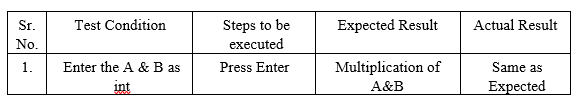
\includegraphics[width=\textwidth]{booth_positive}
\subsection{Negative Testing}
	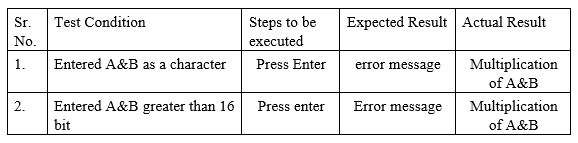
\includegraphics[width=\textwidth]{booth_negative}

\section{Conclusion}
	\paragraph{} We have successfully implemented Booths Multiplication algorithm using BBB modules by building a compute cluster which include availability of low-cost, communitysupported development platform.  
\vspace{20px}
\begin{center}
	\begin{tabular}
		{|c|c|c|c|}\hline
		{\bf Roll No.}		&{\bf Name of Student}		&{\bf Date of Performance}  				&{\bf Date of Submission}  \\ \hline
		{302}	&	{Abhinav Bakshi}& {6/1/16}	&  {20/1/16}\\ \hline
	\end{tabular}\\ 
\end{center}

\section{Plagarism Report}
	 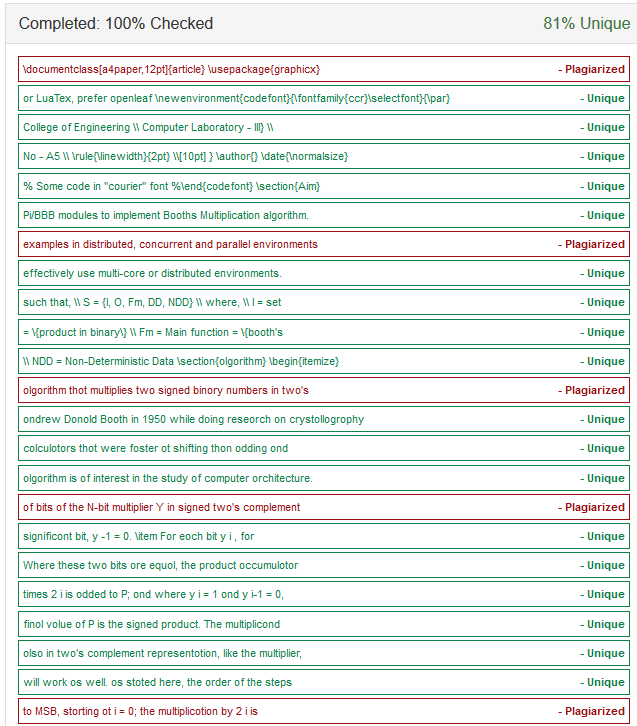
\includegraphics[width=\textwidth]{clusterbooths_plaga}
\end{document}
 

 
